\documentclass[12pt]{article}
\usepackage[margin=1in]{geometry}
\usepackage{natbib}
\usepackage{hyperref}

\usepackage{listings}
\usepackage{rotating, graphicx}
\graphicspath{{./}, {./image/}}
\usepackage{booktabs, natbib}
% \usepackage{breakurl}
% \usepackage [english]{babel}
\usepackage{amsmath, amsbsy, amsthm, epsfig, epsf, psfrag, graphicx, 
amssymb, enumerate}
\usepackage{bm}
\usepackage{multirow, multicol}

\usepackage{color}
\definecolor{darkblue}{rgb}{0.1, 0.2, 0.6}
\usepackage{xcolor}
\newcommand{\jy}[1]{\textcolor{red}{JY: #1}}
\newcommand{\eds}[1]{\textcolor{blue}{(EDS: #1)}}
\newcommand{\mc}[1]{\textcolor{green}{(MC: #1)}}

\sloppy

% \usepackage{csquotes}
% \usepackage [autostyle, english = american]{csquotes}
% \MakeOuterQuote{"}

% \usepackage{bibentry}
\newenvironment{comment}%
{\begin{quotation}\noindent\small\it\color{darkblue}\ignorespaces%
}{\end{quotation}}


\begin{document}

\begin{center}
  {\Large\bf Response to the Comments}
\end{center}


% \jy{Spell check!}

\subsection*{Summary}

We thank the editor and the AE for the opportunity to revise the manuscript and
the two referees for their constructive comments. The manuscript has been
revised accordingly with the following notable changes:
\begin{enumerate}
\item 
  \begin{enumerate}
    \item 
    \item 
    \item 
    \item 
    \end{enumerate}
\item 
  \begin{enumerate}
  \item 
  \item 
  \item 
  \item 
  \end{enumerate}
\end{enumerate}



Point-by-point responses to the comments are as follows, with the
comments quoted in \emph{\color{darkblue} italic}.

\subsection*{To Referee 1}

\begin{comment}
1. It would be helpful to comment on the rationale for the proposed centered CI, 
especially in contrast to why a few others do not work for the log-1 
autocorrelation coefficient.
\end{comment}

After discussion of the flaws of percentile, BC, and BCA CIs at the end of the
first paragraph of Discussion, we have included these additional comments on
why the proposed CI performs well:

The uncertainty measure from bootstrap, which is used to determine the width of
the percentile CI, is quite consistent in comparison to that used for BC and 
BCA CIs. However, for a percentile CI, the center seems
to be at the wrong location but is corrected when $\hat\theta_n$ is used as the
center. This is most likely the reason why the proposed recentered percentile CI
perfoms so much better than percentile, BC, and BCA CIs.

\begin{comment}
2. For all the figures, would it be possible to put the 6 figures in a column in 
a single plot? It would also be helpful to make the figures a bit larger. Right 
now it is hard to compare across different methods regarding their comparative 
performance.
\end{comment}

\begin{figure}[tbp]
  \centering
  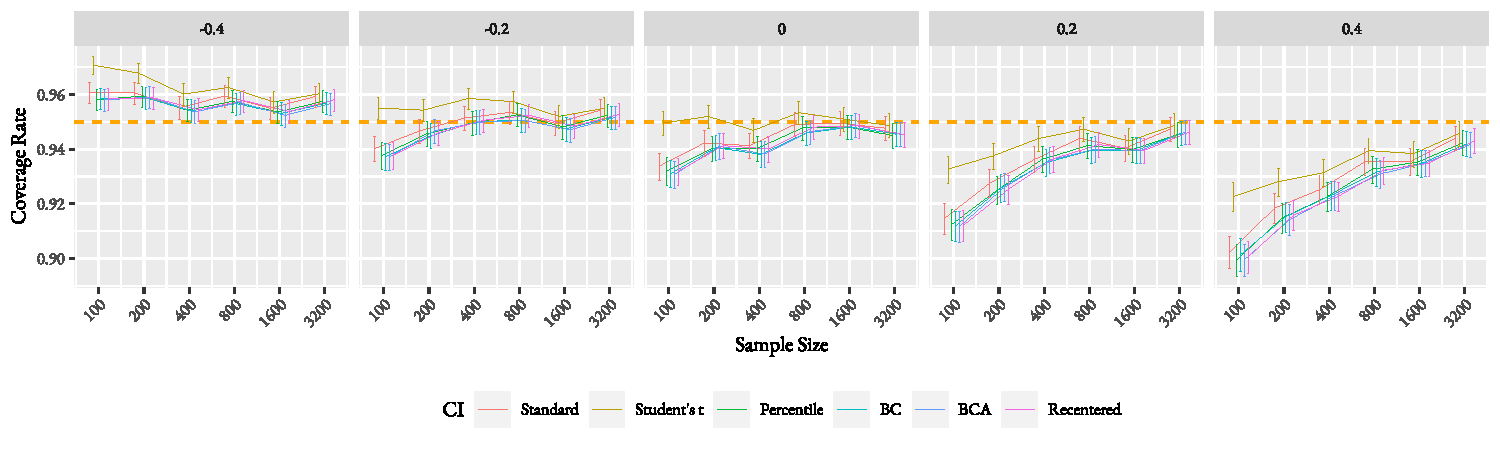
\includegraphics[width=\textwidth]{figures/alt_plot_norm_mu_1}
  \caption{Empirical coverage rates of different 95\% block bootstrap CIs for
    the marginal mean $\mu$ of an AR(1) process with a marginal standard 
    normal distribution with AR coefficient
    $\phi \in \{-0.4, 0.2, 0, 0.2, 0.4\}$ and series length
    $n \in \{100, 200, 400, 800, 1600, 3200\}$ based on 10,000 replicates. The
    error bars represent 95\% CIs of the real coverage rates.}
  \label{fig:mu}
\end{figure}

Here is an example of what this would look like. We find that it is a little
cluttered to make comparisons, so we will use the original format.


\begin{comment}
3. The Appendix should be moved to the main text? Assessing the performance of 
various CI formulations for non-normal error is of central interest.
\end{comment} 

The text from the Appendix has been moved to the Simulation Study section.

\begin{comment}
4. The authors might want to discuss in what circumstances “non-parametric” CI 
formulas would work better. It is a bit surprising that student’s t based 
formula works well under both normal and non-normal error structures.
\end{comment}

The formula for the "parametric" CIs concerns the distribution of the 
bootstrapped statistic, but we actually expect such CIs to work for different
error structures.


\begin{comment}
5. Page 3, 2nd line after “Standard Normal CI”: “p.168” does not seem to fit?
\end{comment}

Because of the style constraints for AJUR, we have removed page numbers in 
citations.

\subsection*{To Referee 2}

\begin{comment}
1. The authors say “....the standard CI is a table-based bootstrap…..”.  
What is meant by “table-based” here?  Is this just a reference to how critical 
values used to be listed in tables?  If that’s the case, I wouldn’t refer to 
this as a “table-based” interval. 
\end{comment}

This terminology was used because, \citet{efron1993introduction} refers to such 
CIs as 
"confidence intervals based on 
bootstrap 'tables'." We have changed these sentences as shown below:

The standard CI is classified by \citet{efron1993introduction} 
as a confidence interval based on bootstrap "tables".
Like the standard normal interval, the
Student's $t$ CI is classified by \citet{efron1993introduction} 
as a confidence interval based on bootstrap "tables".


\begin{comment}
2. Just a comment: The recentered percentile CI proposed here is an interesting 
interval to study. 
\end{comment}

We have added this comment to the discussion:
Lastly, because of its exceptional performance in comparison to the other 
CIs that are not based on bootstrap "tables", the proposed recentered percentile 
CI would be
an interesting method to study further with different bootstrap schemes.

\begin{comment}
3. The sections are numbered, which makes it awkward when the authors refer back 
to a section.  For instance, they refer to “...procedures described in Block 
Bootstrap CIS.”  This would be easier to refer to if the sections were numbered.  
(Is this a journal style choice?  If so, then you can ignore this comment.)
\end{comment}

This is a journal style choice.

\begin{comment}
4.  In Figure 1 (and all the other figures), the authors present confidence 
intervals for the real coverage rates.  The authors should specify what type of 
CI they are using here.  I assume the authors are using a Wald-type interval for 
this CI as this is for a proportion.  If that’s the case, it’s well known that 
the Wald-type interval has undercoverage when the true proportion is near 0 or 
1, which is the case in several of these scenarios, especially when phi is -0.4. 
\end{comment}

We modified the Design section as below:

If all values in the interval are below 0.95, the results would suggest 
that the method either is providing inaccurate estimation, is underestimating 
the process' variability, or a combination of both. If all values in the 
interval are above .95, the results suggest that the method is overestimating 
the process' variability. \citet{brown2001interval} notes that the Wald-type 
interval has poor coverage as the proportion approaches 0 or 1.

\begin{comment}
5.  In all the figures, the y-axis is allowed to vary freely making it hard to 
compare one row directly to another.  I would suggest fixing the limits on the 
y-axis to make comparisons easier.  
\end{comment}

Because of the deterioration for $\phi$, we found it hard to fix the limits on 
the 
y-axis without hurting the visualization for the other rows. Below is an 
example:

\begin{figure}[tbp]
  \centering
  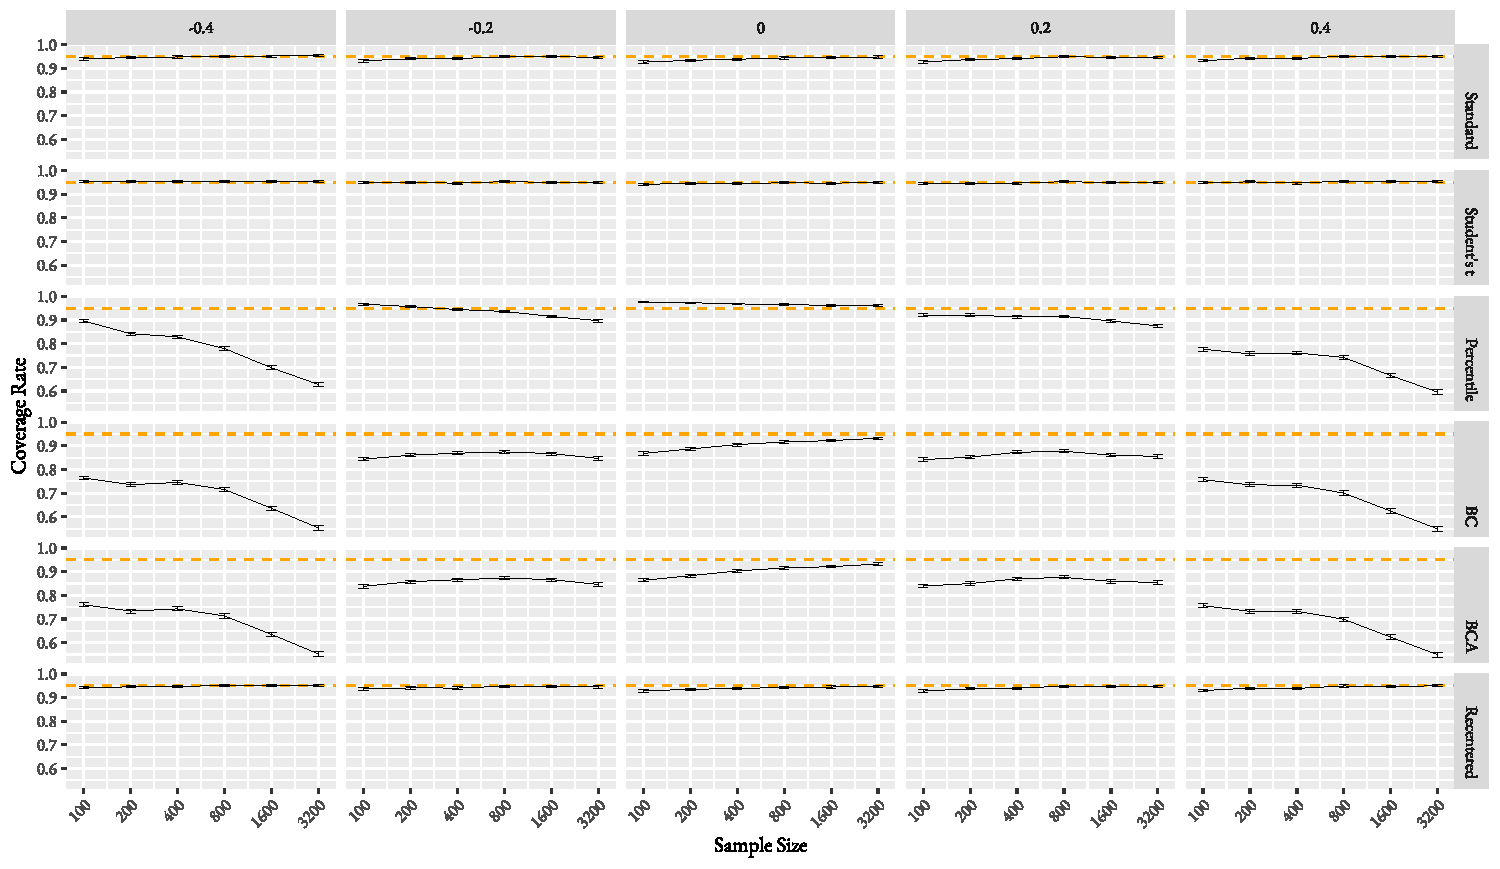
\includegraphics[width=\textwidth]{figures/alt2plot_norm_phi_1}
  \caption{Empirical coverage rates of different 95\% block bootstrap CIs for 
    the first-order autocorrelation coefficient $\phi$ of an AR(1) process with 
    a marginal standard normal distribution with 
    $\phi \in \{-0.4, 0.2, 0, 0.2, 0.4\}$ and series length
    $n \in \{100, 200, 400, 800, 1600, 3200\}$ based on 10,000 replicates of
    block bootstrap with $l = \lceil n^{1/3} \rceil$. The
    error bars represent 95\% CIs of the real coverage rates.}
  \label{fig:phi1}
\end{figure}

\begin{comment}
6.  Is there a reason why the coverage for mu (in Figure 1) is better for 
negative autoregressive terms when compared with the positive autoregressive 
term? Can the authors give some intuition behind why that makes sense? 
\end{comment}

- When there is a positive correlation, effective sample size is lesser
- When there is a negative correlation, effective sample size is larger, 
meaning the coverage is better

\begin{comment}
7.  The authors say “A smaller sample size is generally required to estimate a 
parameter for a sample with a negative phi versus a positive phi of the same 
magnitude.”  On a quick reading of this it sounds like the authors are 
recommending using a smaller sample size when phi is negative.  I believe what 
you are trying to say is that coverage rates are acceptable at smaller sample 
sizes when phi is negative versus when phi is positive (i.e. it takes larger 
sample sizes to get acceptable coverage when phi is positive).  Change this 
sentence to make it more clear. 
\end{comment}

The original sentence has been replaced with:
Coverage rates are acceptable at smaller sample 
sizes when phi is positive versus when phi is negative. In
other words, a larger sample size is generally required to estimate a 
parameter for a sample with a negative $\phi$ versus a positive $\phi$ of the 
same magnitude.

\begin{comment}
8.   In the Discussion section, the authors say “We know theoretically that the 
block bootstrap procedure will cover the parameter of a time series given an 
infinitely large sample.”  Essentially, you are stating that the estimator is 
consistent.  Is there a citation that you can point to that shows that this is 
true? 
\end{comment}

\citep{calhoun2018}

\begin{comment}
9.   The authors studied coverage rates of the different intervals as a function 
of sample size, but they only looked at one choice for the number of blocks.  
Why did the authors choose to not also look at how the number of blocks affects 
the coverage rates?
\end{comment}

We have now repeated the same simulation study with block size as an 
additional experimental factor. The optimal order of block size is 
$\lceil n^{1/3} \rceil$, so we tried the same simulations using 
$l = \lceil n^{1/3} \rceil$ and $l = \lceil 2n^{1/3} \rceil$


\begin{comment}
10.   Why did the authors choose to only go as high as 0.4 (and as low as -0.4) 
for the autocorrelation parameter?  I would think that these correlations near 1 
(or -1) would be some of the more interesting cases to study, but they are 
completely ignored here.  Can the authors justify their choice to leave it out 
of this study?
\end{comment}

For practical purposes, it is in fact rare for autocorrelations to be stronger
than 0.4. We have established the trend as the strength of the autocorrelation 
increases, and how it varies depending on the sign of the autocorrelation and 
the parameter of interest.

\begin{comment}
11.    Last paragraph: The authors mention the “ABC and bootstrap-t intervals”.  
They do not give a citation for these intervals.   Add a citation. 
\end{comment}

These intervals are discussed in \citep{efron1993introduction}. A citation
is now provided in the last paragraph.



\begin{comment}
12.    The last line of the manuscript offers one line about the drawbacks of 
the block bootstrap almost as an afterthought.  I think a discussion of the 
drawbacks should be expanded and added to the introduction as this is an 
important point that isn’t mentioned at all until the literal last line. 
\end{comment}

We have included this discussion of problems with block bootstrap in the
introduction:

\citet{lahiri1999theoretical} finds that moving block bootstrap has better 
performance than non-overlapping block bootstrap. Additionally, moving block 
bootstrap with nonrandom
block sizes results in lower mean-squared errors than moving block bootstrap
with random block sizes. \citet{buhlmann1999block} notes that a drawback of 
block bootstrap is that it heavily depends on block size, which has to be chosen
by the user of the method.
Even when using the appropriate settings, as noted by
\citet{buhlmann2002bootstraps} notes some general drawbacks of block 
bootstrap --- with respect to how reasonably it imitates the data-generating 
process. In addition, although block bootstrap is primarily used for stationary 
time series, it can be outperformed by other bootstrap schemes for linear time
series and categorical processes.


We are indebted to the reviewers for pointing out these vital discussion areas,
which have not only enriched the current paper but also charted a clear course
for our subsequent research endeavors.


\bibliographystyle{chicago}
\bibliography{citations}


\end{document}
